\section{Additional high-dimensional regression study}

At the request of the referees, we conducted an additional simulation study in a simple regression setting without treatment assignment or censoring. 
The goal of this experiment is to allow for a clean comparison of shrinkage mechanisms within Bayesian tree ensembles. 
Accordingly, we restrict attention to Bayesian tree-based methods and do not include comparisons with non-Bayesian competitors such as random forests, boosting, or MARS. 
The focus is solely on how different regularisation strategies behave in high-dimensional non-linear regression.
The following simulations are inspired on the simulations performed by \citet{linero2018dirichlet} and \citet{LineroYang2018}.

Let $Y_i$ denote a continuous outcome and $X_i$ a $p$-dimensional covariate vector. 
We consider a single-forest tree ensemble model in which the outcome is represented as a noisy sum of regression trees:
\begin{equation}\label{bart_model}
Y_i = \sum_{j=1}^m g(X_i; \mathcal{T}_j, \mathcal{H}_j) + \varepsilon_i, 
\qquad 
\varepsilon_i \sim \mathcal{N}(0, \sigma^2),
\end{equation}
where each $\mathcal{T}_j$ is a binary decision tree defining recursive partitioning rules over the covariate space, and 
$\mathcal{H}_j = \{h_{j1}, \ldots, h_{jL_j}\}$ denotes the set of step heights associated with the $L_j$ terminal nodes of tree $\mathcal{T}_j$.
The function $g$ maps a covariate vector $X_i$ to the corresponding leaf-specific step height determined by the tree structure $\mathcal{T}_j$ and its associated parameters $\mathcal{H}_j$. 
That is, $g(X_i; \mathcal{T}_j, \mathcal{H}_j) = h_{jl}$ if $X_i$ falls into terminal node $l$ of tree $\mathcal{T}_j$.

We compare the following Bayesian tree ensemble methods, each of which induces a different form of regularisation:



\begin{itemize}

\item \textbf{BART} \citep{BARToriginal}.  
Regularisation is primarily imposed through the tree-structure prior, which penalises deep trees, and through Gaussian priors on the step heights $h_{jl}$. 
Shrinkage is global and homogeneous across leaves.

\item \textbf{DART} \citep{linero2018dirichlet}.  
Extends BART by placing a Dirichlet prior on splitting probabilities. 
This induces sparsity at the covariate-selection level by encouraging splits to concentrate on a subset of predictors.

\item \textbf{SoftBART} \citep{LineroYang2018}.  
Replaces hard splits with smooth gating functions and learns splitting weights adaptively. 
Regularisation is achieved through both smooth decision rules and hierarchical shrinkage on step heights.

\item \textbf{Horseshoe Forest} \citep{main_article}  
We use a single forest with a horseshoe global--local prior on the step heights.
Specifically, each step height is assigned a local shrinkage parameter while a tree-specific global shrinkage parameter controls overall regularisation. 
The default shrinkage level $k=0.1$ is used throughout. 


\end{itemize}


For each individual $i = 1,\ldots,n$, we generate data according to
\begin{equation}
\begin{split}
    X_i &\sim \mathcal{U}[0,1]^p, \\
    \beta &\sim (1-s)\delta_{0_p} + s\,\mathcal{N}(0_p, I_p), \\
    f(x_i) &= 10 \sin(\pi x_{i1} x_{i2})
             + 20 (x_{i3} - 0.5)^2\\
             &\quad\quad + 10 x_{i4}
             + 5 x_{i5}
             + x_i^\top \beta, \\
    Y_i &\sim \mathcal{N}\big(f(x_i),\, \sigma^2\big),
\end{split}
\end{equation}
where $s = 0.05$ denotes the sparsity level. 
Each coefficient $\beta_j$ is drawn independently from a spike-and-slab distribution: it equals zero with probability $1-s$ and is sampled from a standard normal distribution with probability $s$.
The signal consists of a fixed non-linear component \citep{Friedman} depending on the first five covariates, and a sparse high-dimensional linear term $x_i^\top \beta$ with  sparsity level $s=0.05$. 
We set $\sigma^2$ such that $\mathrm{var}(Y)/\sigma^2 = 1.11\overline{1}$.


We first consider covariate dimensions $p \in \{500, 1000, 5000\}$ while fixing the sample size at $n = 100$. For each setting, we report the root mean squared error (RMSE), empirical coverage of the 95\% credible prediction intervals, and the average interval length.
Secondly, we investigate the high-dimensional behaviour in more detail by incrementally increasing $p$ from 50 to 5000. 
We plot the RMSE and empirical coverage of the posterior predictive intervals as functions of the covariate dimension $p$.

\subsection{Results}

\begin{figure}[tb]
\centering
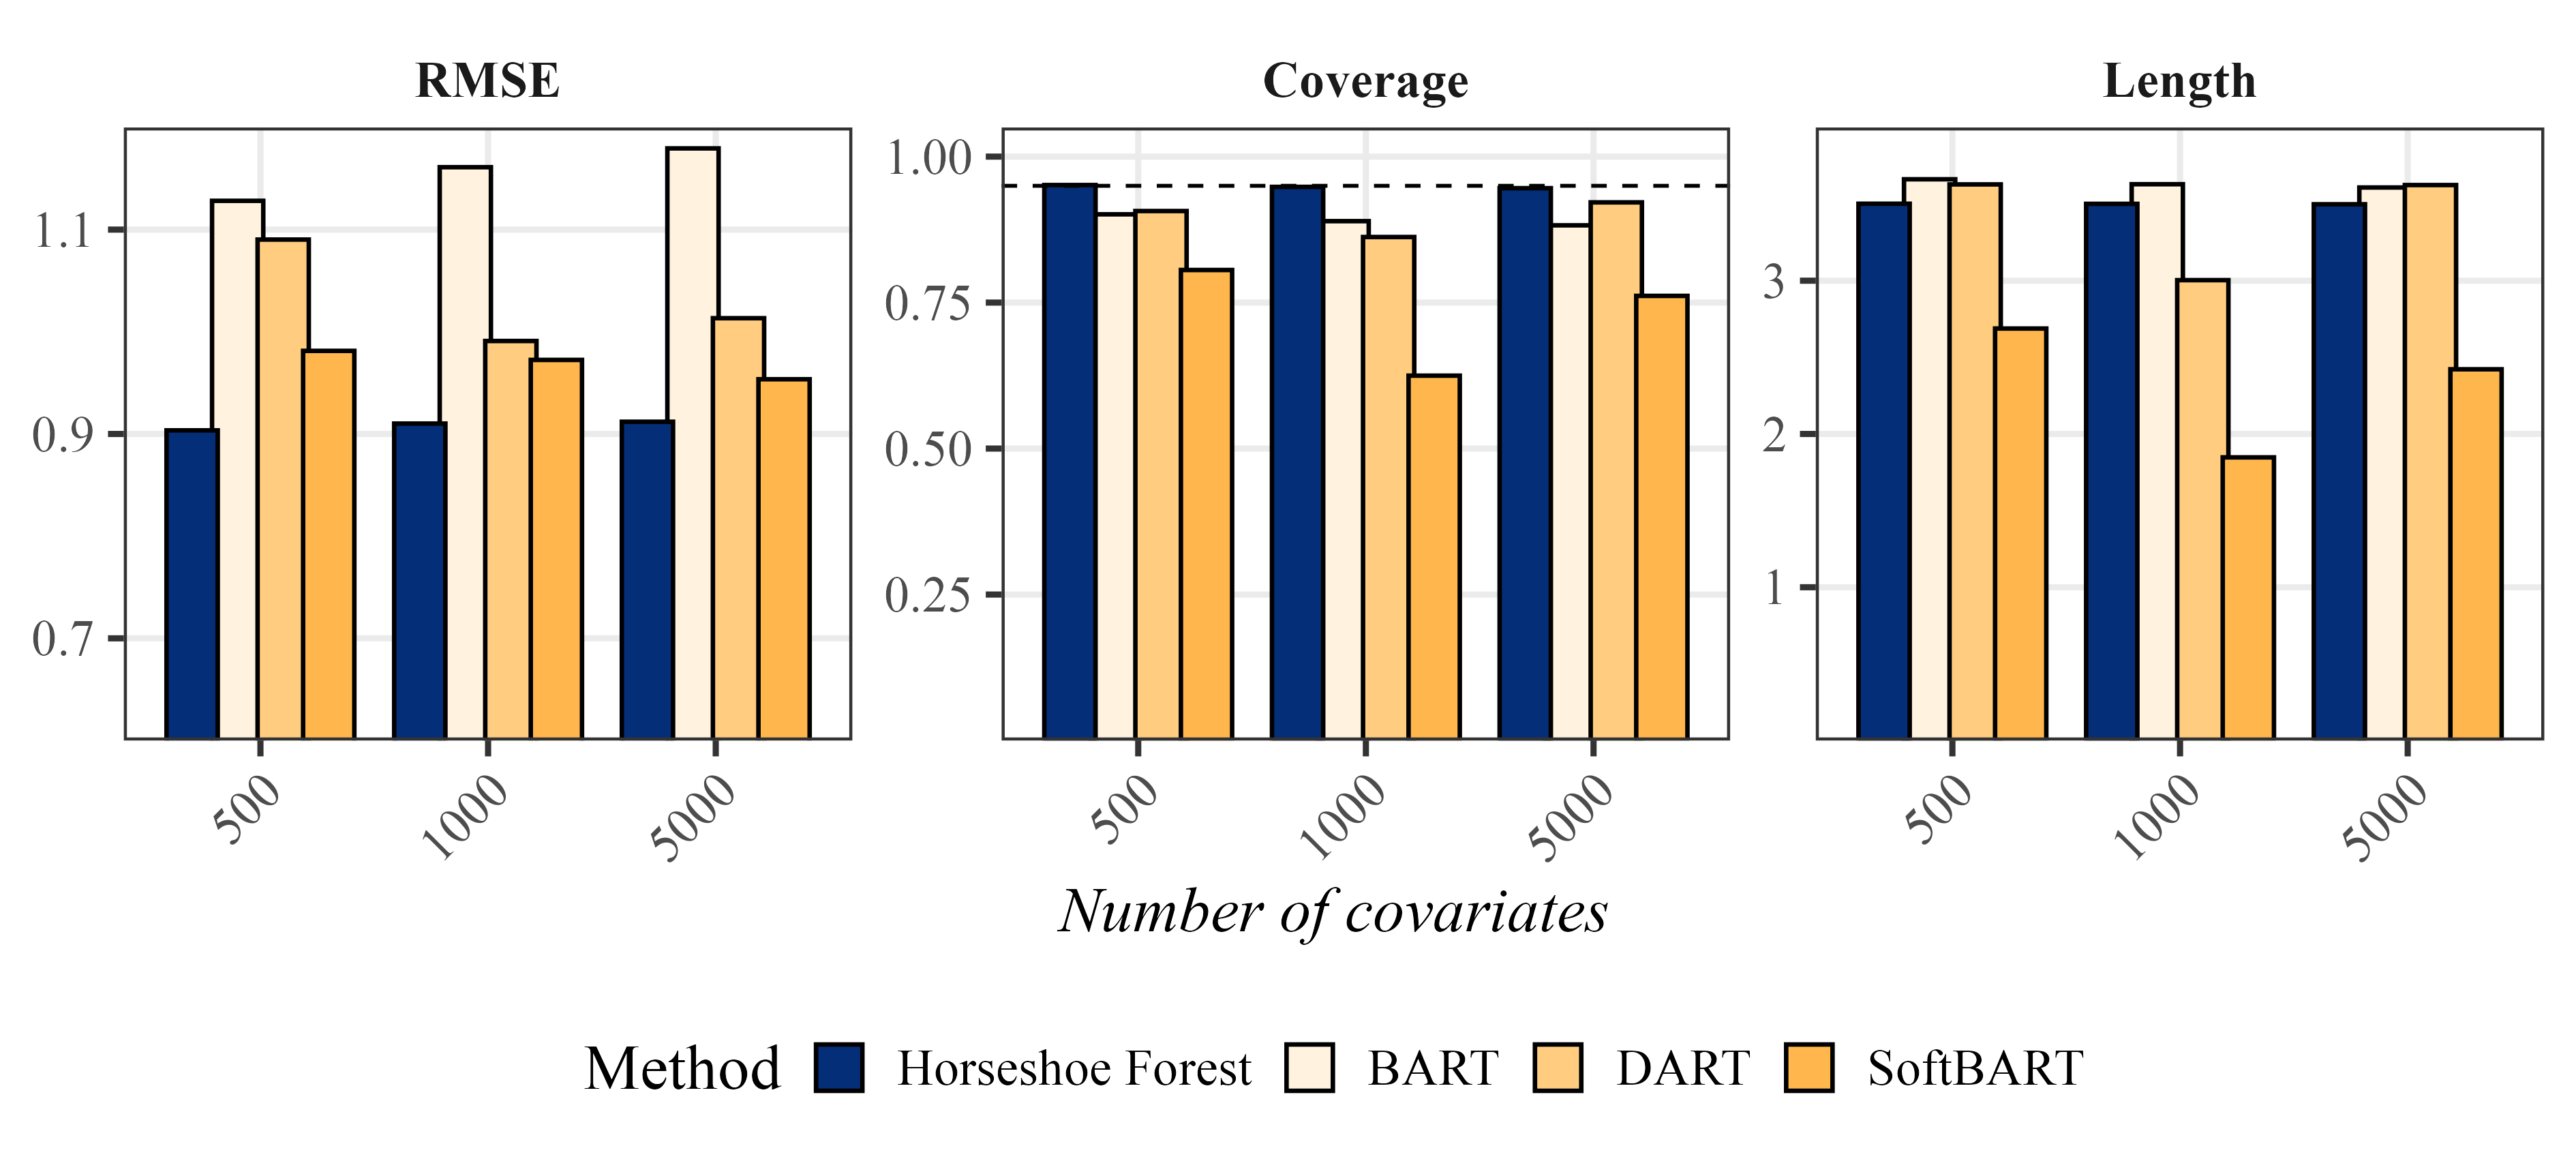
\includegraphics[width=\linewidth]{revision_simple_bar_plot.png}
\caption{
Performance comparison of Bayesian tree ensemble methods in a simple regression setting.
We report the root mean squared error (RMSE), empirical coverage of the 95\% posterior credible intervals, and the average credible interval length.
}
\label{fig:revision_simple_regression}
\end{figure}

The results for the settings $p \in \{500,1000,5000\}$ are shown in Figure~\ref{fig:revision_simple_regression}.
The Horseshoe Forest achieves the lowest RMSE across all three dimensions. 
Its predictive accuracy remains stable as $p$ increases. 
Standard BART yields consistently higher RMSE and does not improve with increasing $p$. DART and SoftBART reduce the error relative to BART.

The Horseshoe Forest attains empirical coverage close to the nominal $95\%$ level across all covariate dimensions while keeping interval lengths moderate. 
Standard BART achieves similar coverage but produces slightly wider intervals. 
DART shows some undercoverage, particularly in higher dimensions. 
SoftBART produces the shortest intervals but suffers from substantial undercoverage.


\begin{figure}[b!]
    \centering
    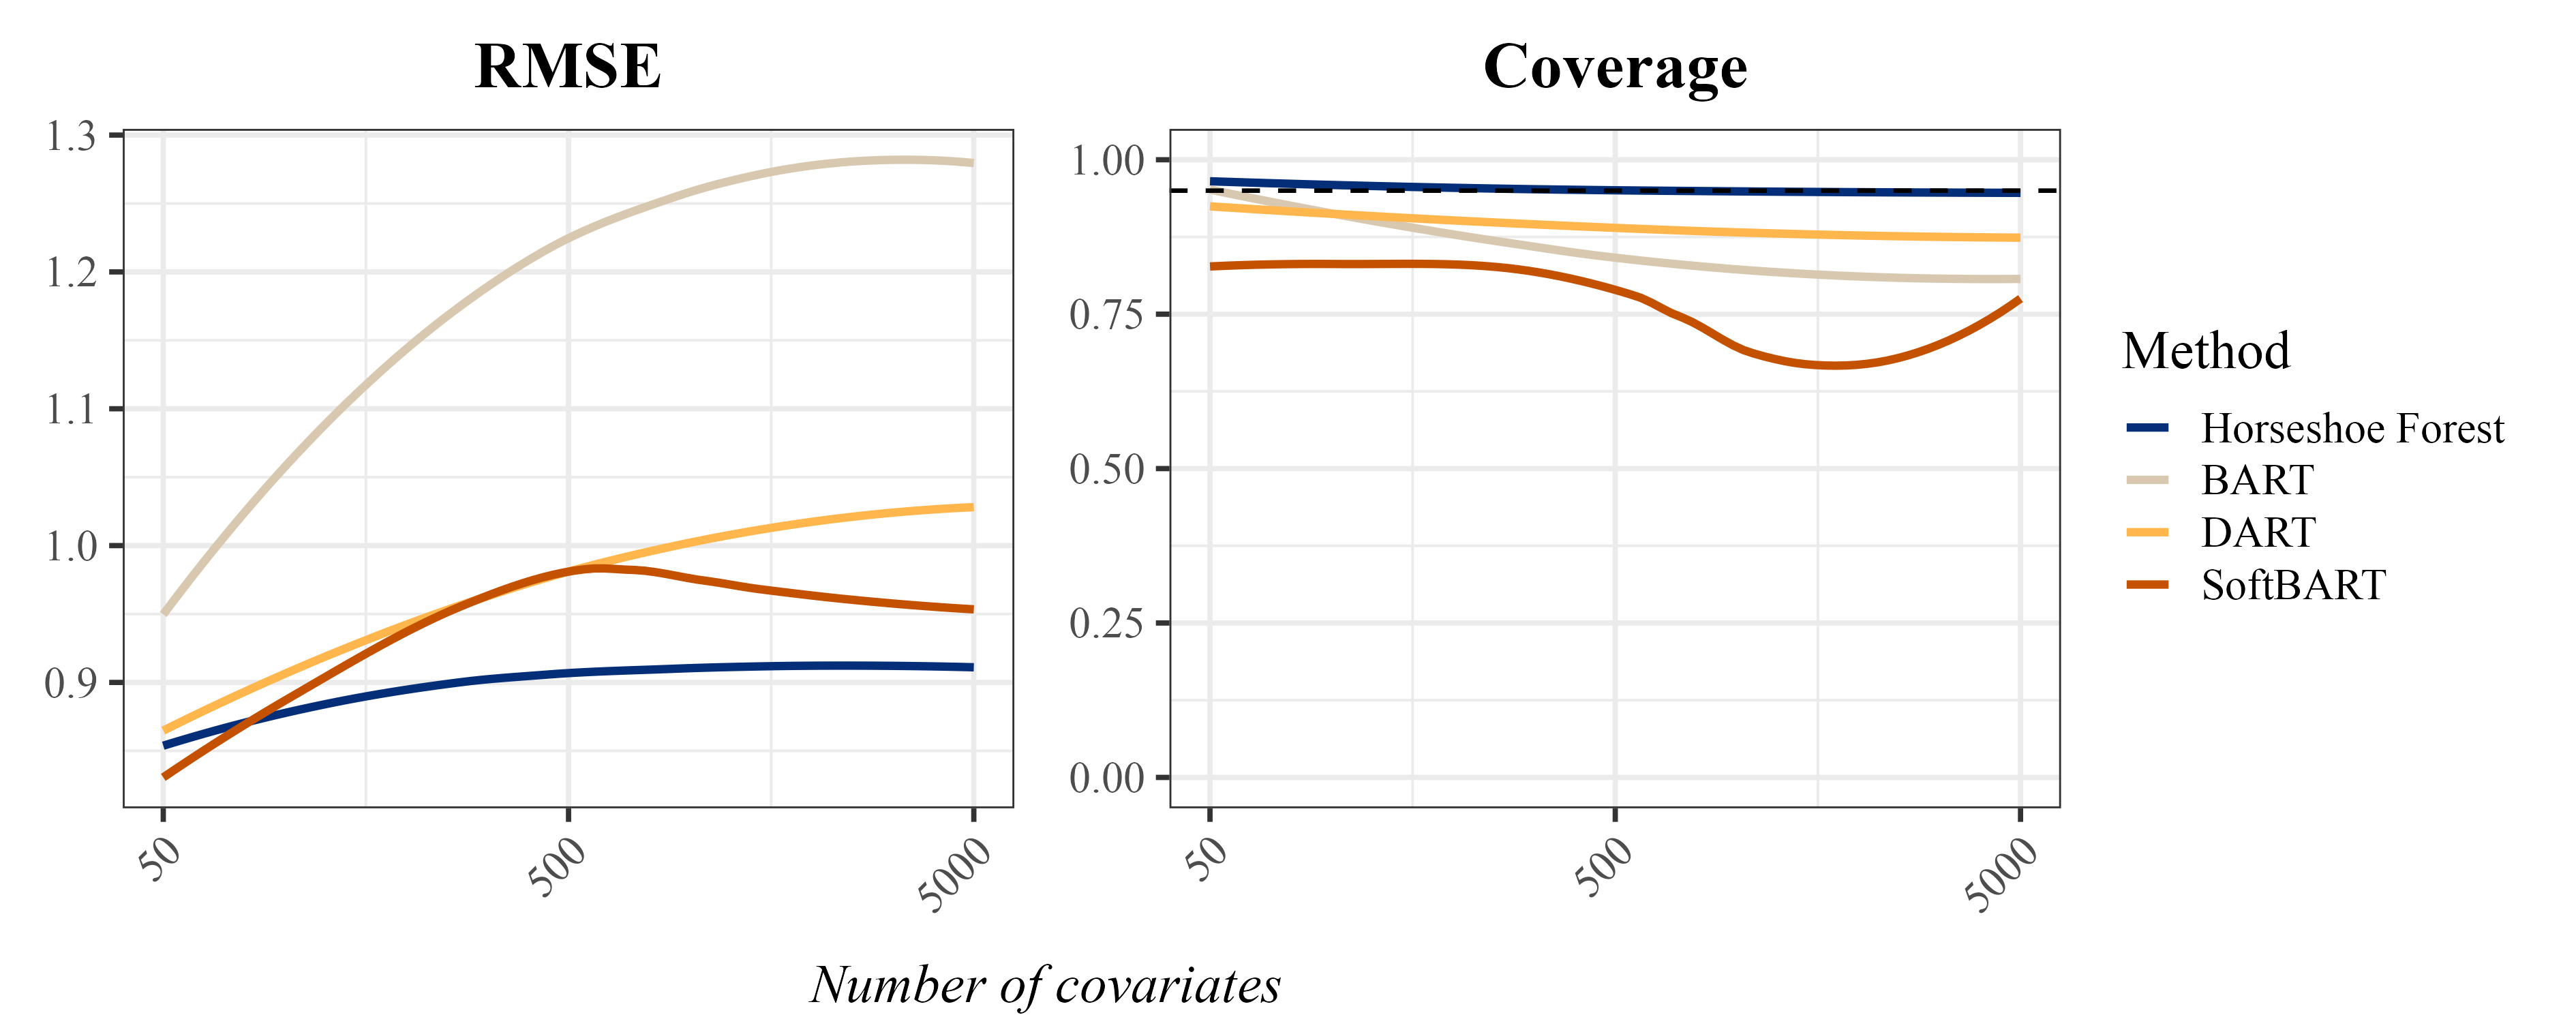
\includegraphics[width=\linewidth]{revision_simple_deeper_plot.png}
    \caption{
    Performance comparison of Bayesian tree ensemble methods in a high-dimensional regression setting.
    The left panel shows the root mean squared error (RMSE) and the right panel shows the empirical coverage of 95\% posterior credible intervals as a function of the number of covariates $p$.
    }
    \label{fig:revision_simple_deeper}
\end{figure}

The results for $p$ varying from $50$ to $5000$ are shown in Figure~\ref{fig:revision_simple_deeper}. 
The Horseshoe Forest exhibits stable predictive accuracy across the entire range and achieves the lowest RMSE in moderate to high dimensions. 
Standard BART consistently shows the highest prediction error. 
DART improves upon standard BART and shows a noticeable gain in predictive accuracy once $p$ exceeds approximately $500$. 
SoftBART performs competitively in low dimensions, with relatively small prediction error when $p$ is close to $50$. 
As dimensionality increases, its RMSE rises in the moderate regime and then decreases slightly for larger $p$, leading to a mildly non-monotone pattern. 
The predictive performance of SoftBART remains between that of DART and the Horseshoe Forest in higher dimensions.

Coverage of the Horseshoe Forest remains close to the nominal $95\%$ level throughout. 
BART and DART shows moderate undercoverage at intermediate dimensions. 
SoftBART shows undercoverage 
SoftBART exhibits more pronounced undercoverage across most of the range. 
Its coverage declines further in the moderate-dimensional regime and only partially recovers for larger $p$, remaining below nominal. 

SoftBART displays mildly non-monotone behaviour in both RMSE and coverage as $p$ increases, with visible local fluctuations in the moderate-dimensional regime. 
Additional simulation runs confirm that this pattern is reproducible and not driven by Monte Carlo noise. 
While SoftBART remains computationally feasible across the considered dimensions, its runtime increases more markedly with $p$ than that of the Horseshoe Forest, reflecting the additional complexity of its soft splitting mechanism.

